\section{Project results}
After have done the implementaion we've been making some measurements with our
temperature sensor mote. From these measurements there is made a single graph,
\ref{fig:results} with shows the sensor's temperature. The figure show also
that, as earlier described that the temperature is multiplied by $100$.
Therefore it's clear to see that the data in the figure are more fine grain in
the graph, and it gives a more linear impression.
\begin{landscape}
\begin{figure}[htbp]
\begin{center}
	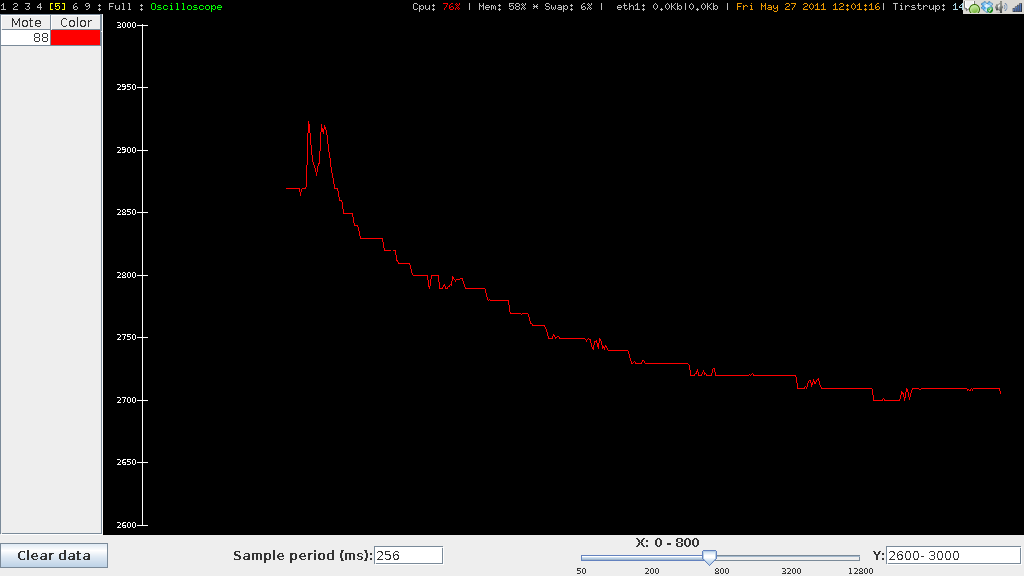
\includegraphics[width=26cm,trim={0 0 0 14},clip=true]{img/graph}
\caption{A graph which consists of periodically temperature measurements made by the temperature sensor mote}
\label{fig:results}
\end{center}
\end{figure}
\end{landscape}
